\documentclass[12pt]{tdtp}
\usepackage{tabularx,colortbl}
\usepackage{multirow}
\usepackage{listings}
\lstset{
	language=VHDL,
basicstyle=\tiny\ttfamily}
\definecolor{light-gray}{gray}{0.96}
\definecolor{pageheading-gray}{gray}{0.2}
\definecolor{dark-gray}{gray}{0.45}
\definecolor{dark-green}{rgb}{0.245,0.121,0.0}

\newcommand{\auteur}{Cedric Lemaitre}
\newcommand{\couriel}{c.lemaitre58@gmail.com}
\newcommand{\promo}{Bachelor in Computer Vision}
\newcommand{\annee}{2016-2017}
\newcommand{\matiere}{Image Processing}

\newcommand{\tdtp}{Labs 2}
\renewcommand{\sujet}{Image filtrering and histogram}


\begin{document}
\titre

%%%%%%%%%%%%
\Exo

In this exercise we consider the following image \textit{the galaxy} (figure : \ref{Galaxy}).\\
Test on this image the following alogrithms: Robert gradient, Sobel gradient, Laplacian.\\
Join a copy of your Matlab code in the report.


\begin{figure}[h!]
	\begin{center}
		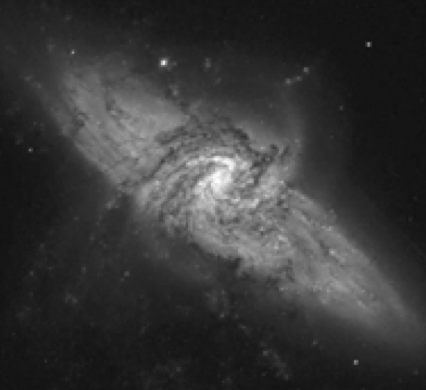
\includegraphics[scale=0.5]{images/galaxy.png}
		\caption{Test image}
		\label{Galaxy}
	\end{center}
\end{figure}

%%%%%%%%%%%%
\newpage 
\Exo


Add a gaussian white noise on the image (figure : \ref{Galaxy}) and then use a spatial low-pass filter to eleminate the artefacts.\\
Give the measure of the PSNR of the image with noise and of the filtered image.\\
Then on the original image use a spatial high-pass filter on the originalimage to enhanced the transitions.\\
Join a copy of your Matlab code in the report.
%%%%%%%%%%
\newpage 
\Exo
Enhance the contrast on the scan image (figure : \ref{mri}).
Join a copy of your Matlab code.

\begin{figure}[h!]
	\begin{center}
		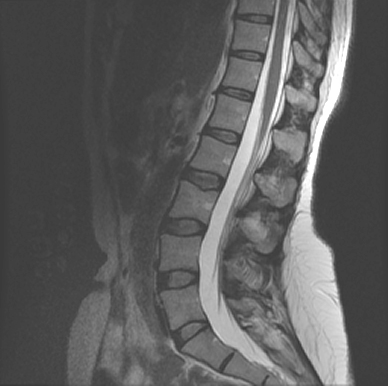
\includegraphics[scale=0.5]{images/mri.png}
		\caption{Scan Image}
		\label{mri}
	\end{center}
\end{figure}


%%%%%%%%%%%%%%%%%%%%%%%%%%%%%%%%%%
\end{document}
